\begin{frame}{Monte Carlo integration}
\begin{center}
$
\ds \int_a^b f(x) dx \approx \frac{b-a}{N} \sum_{i=1}^N f(X_i), \;
$
where $X \sim Uniform(a,b)$
\end{center}

\begin{itemize}
\item[\tickYes] Convergence rate independent of the dimension: $\mathcal{O}(N^{-1/2})$
\item[\tickNo] Slow convergence in low dimensions (1D, 2D, 3D)
\item[\tickYes] Appropriate for high dimensions
\item[\tickYes] Mesh-free method
\item[\tickYes] Allows the use of autodiff to compute $\nabla u$
\item[\tickYes] Easy to implement
\item[\tickYes] Exploit the use of minibatches and GPUs
\end{itemize}
\end{frame}


\begin{frame}{Explainability of the NN: Regularization methods}
\centering

\begin{itemize}
\item We  minimise the loss:
$$\mathcal{L}_{total} = \mathcal{L}_{Ritz}+R.$$
\vspace{0.2cm}

\item Using arguments similar to (Mishra \textit{et al.}, 2020), we define $R$ for a simple NN as:

\begin{equation*}
R\left(\theta, u_{NN}(x_i), \dfrac{\partial^{n}u_{NN}(x_i) }{\partial x^{n}} \right).
\end{equation*}


\vspace{0.2cm}
\item $R$ acts as a regularizer, penalising poor quadrature via the loss. 
%\vspace{0.2cm}
%\item $\mathcal{R}\sim \frac{1}{N}$, so for $N$ large, the ``bias" from $\mathcal{R}$ vanishes.
%

\vspace{0.5cm}

%\beamertemplatebookbibitems
\begin{thebibliography}{1}
%\bibitem{Author1990}A. Author. \newblock\emph{Handbook of Everything}.\newblock
%Some Press, 1990.\beamertemplatearticlebibitems
\bibitem{Mishra}Mishra, S., Molinaro, R.: Estimates on the generalization error of physics informed neural
networks (PINNs) for approximating PDEs. ArXiv:2006.16144 (2020).
\end{thebibliography}
\end{itemize}
\end{frame}


\begin{frame}{Explainability of the NN: Regularization methods}
\vspace{0.25cm}
\begin{itemize}
\item[\tickYes]The loss prohibits overfitting
\vspace{0.15cm}

\item[\tickYes] We have {\it a posteriori} estimation of quadrature error
\vspace{0.15cm}

\item[\tickYes] $R$ is computationally cheap to evaluate
\vspace{0.15cm}
%
%\item[\tickNo] If $N$ is small, the problem is drastically changed by $R$
%\vspace{0.15cm}

\item[\tickNo] Finding an expression for $R$ is difficult and problem dependent
\vspace{0.15cm}

\item[\tickNo] Only valid for regular integrands
\end{itemize}
\end{frame}


\begin{frame}{Adaptive Integration}
\only<1-1>{
\centering
\begin{columns}
\begin{column}{0.7\textwidth}
	\begin{figure}[!htp]
		\begin{tikzpicture}
% TRAIN
\node at (1,1) {};
\node at (1,-4) {};

\draw[<->, dashed] (0,0.5) -- (2,0.5);
\node at (1,0.75) {$h$};
\draw (0,0) -- (8,0);
\foreach \Point in {(0,0), (2,0), (4,0), (6,0), (8,0)}{\node at \Point {\textbullet};}
\node at (0,-0.25) {$a$};
\node at (8,-0.25) {$b$};


% VALIDATION
\draw[<->, dashed] (0,-3.5) -- (1,-3.5);
\node at (0.5,-3.75) {$h/2$};

\draw (0,-3) -- (8,-3);
\foreach \Point in {(0,-3), (2,-3), (4,-3), (6,-3), (8,-3)}{\node at \Point {\textbullet};}
\foreach \Point in {(1,-3), (3,-3), (5,-3), (7,-3)}{\node[blue] at \Point {\textbullet};}
\node at (0,-3.25) {$a$};
\node at (8,-3.25) {$b$};

\end{tikzpicture}
		\label{fig:adaptive_1}
 	\end{figure}
\end{column}

\begin{column}{0.3\textwidth}
Training set

\vspace{2.5cm}

Validation set
\end{column}
\end{columns}
 }

\only<2-2>{
\centering
\begin{columns}
\begin{column}{0.7\textwidth}
	\begin{figure}[!htp]
		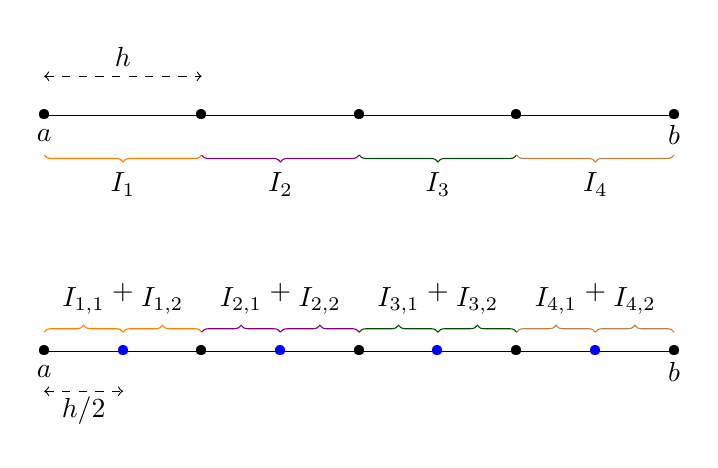
\begin{tikzpicture}
\node at (1,1) {};
\node at (1,-4) {};
% TRAIN
\draw[<->, dashed] (0,0.5) -- (2,0.5);
\node at (1,0.75) {$h$};
\draw (0,0) -- (8,0);
\foreach \Point in {(0,0), (2,0), (4,0), (6,0), (8,0)}{\node at \Point {\textbullet};}
\node at (0,-0.25) {$a$};
\node at (8,-0.25) {$b$};

\draw [orange, decorate, decoration = {brace,mirror}] (0,-0.5) -- (2,-0.5)node[pos=0.5,below=3pt,black]{$I_{1}$};

\draw [violet, decorate, decoration = {brace,mirror}] (2,-0.5) -- (4,-0.5)node[pos=0.5,below=3pt,black]{$I_{2}$};

\draw [green!30!black, decorate, decoration = {brace,mirror}] (4,-0.5) -- (6,-0.5)node[pos=0.5,below=3pt,black]{$I_{3}$};

\draw [brown, decorate, decoration = {brace,mirror}] (6,-0.5) -- (8,-0.5)node[pos=0.5,below=3pt,black]{$I_{4}$};

% VALIDATION
\draw[<->, dashed] (0,-3.5) -- (1,-3.5);
\node at (0.5,-3.75) {$h/2$};

\draw (0,-3) -- (8,-3);
\foreach \Point in {(0,-3), (2,-3), (4,-3), (6,-3), (8,-3)}{\node at \Point {\textbullet};}
\foreach \Point in {(1,-3), (3,-3), (5,-3), (7,-3)}{\node[blue] at \Point {\textbullet};}
\node at (0,-3.25) {$a$};
\node at (8,-3.25) {$b$};

\draw [orange, decorate, decoration = {brace}] (0,-2.75) -- (1,-2.75)node[pos=0.5,above=3pt,black]{$I_{1,1}$};
\draw [orange, decorate, decoration = {brace}] (1,-2.75) -- (2,-2.75)node[pos=0.5,above=3pt,black]{$I_{1,2}$};
\node at (1, -2.25) {$+$};
%\node at (1, -1.55) {\textcolor{red}{$\approx$?}};

\draw [violet, decorate, decoration = {brace}] (2,-2.75) -- (3,-2.75)node[pos=0.5,above=3pt,black]{$I_{2,1}$};
\draw [violet, decorate, decoration = {brace}] (3,-2.75) -- (4,-2.75)node[pos=0.5,above=3pt,black]{$I_{2,2}$};
\node at (3, -2.25) {$+$};
%\node at (3, -1.55) {\textcolor{red}{$\approx$?}};

\draw [green!30!black, decorate, decoration = {brace}] (4,-2.75) -- (5,-2.75)node[pos=0.5,above=3pt,black]{$I_{3,1}$};
\draw [green!30!black, decorate, decoration = {brace}] (5,-2.75) -- (6,-2.75)node[pos=0.5,above=3pt,black]{$I_{3,2}$};
\node at (5, -2.25) {$+$};
%\node at (5, -1.55) {\textcolor{red}{$\approx$?}};

\draw [brown, decorate, decoration = {brace}] (6,-2.75) -- (7,-2.75)node[pos=0.5,above=3pt,black]{$I_{4,1}$};
\draw [brown, decorate, decoration = {brace}] (7,-2.75) -- (8,-2.75)node[pos=0.5,above=3pt,black]{$I_{4,2}$};
\node at (7, -2.25) {$+$};
%\node at (7, -1.55) {\textcolor{red}{$\approx$?}};
\end{tikzpicture}
		\label{fig:adaptive_1}
 	\end{figure}
\end{column}

\begin{column}{0.3\textwidth}
Training set

\vspace{2.5cm}

Validation set
\end{column}
\end{columns}
 }

\only<3-3>{
\centering
\begin{columns}
\begin{column}{0.7\textwidth}
	\begin{figure}[!htp]
		\input{Diapos/PDEs_with_NN/Figures/Quadrature_problem/Adaptive/Adaptive_3b.tex}
		\label{fig:adaptive_1}
 	\end{figure}
\end{column}

\begin{column}{0.3\textwidth}
Training set

\vspace{2.5cm}

Validation set
\end{column}
\end{columns}
 } 

\only<4-4>{
\centering
\begin{columns}
\begin{column}{0.7\textwidth}
	\begin{figure}[!htp]
		\input{Diapos/PDEs_with_NN/Figures/Quadrature_problem/Adaptive/Adaptive_4b.tex}
		\label{fig:adaptive_1}
 	\end{figure}
\end{column}

\begin{column}{0.3\textwidth}
Training set 

\vspace{2.5cm}

Validation set
\end{column}
\end{columns}
 }

\only<5-5>{
\centering
\begin{columns}
\begin{column}{0.7\textwidth}
	\begin{figure}[!htp]
		\input{Diapos/PDEs_with_NN/Figures/Quadrature_problem/Adaptive/Adaptive_5b.tex}
		\label{fig:adaptive_1}
 	\end{figure}
\end{column}

\begin{column}{0.3\textwidth}
Training set 

\vspace{2.5cm}

Validation set
\end{column}
\end{columns}
 } 
\end{frame}


\begin{frame}{Adaptive Integration}
\vspace{0.25cm}
\begin{itemize}
\item[\tickNo] Mesh based
\vspace{0.15cm}

\item[\tickYes] Appropiate for low dimensional problems
\vspace{0.15cm}

\item[\tickYes] Allows the use of autodiff to compute $\nabla u$
\vspace{0.15cm}
\end{itemize}
\end{frame}


\begin{frame}{Piecewise-polynomial approximation}

%\begin{itemize}
%\item We define a mesh
%\end{itemize}
%
%\begin{center}
%\begin{tikzpicture}
%\draw (0,0) -- (8,0);
%\draw[red,fill=red] (0,0) circle (0.7ex);
%\draw[violet,fill=violet] (8,0) circle (0.7ex);
%\node [red] at (0,-0.4){$\Gamma_D$};
%\node [violet] at (8,-0.4){$\Gamma_N$};
%%
%\foreach \Point in {(2,0), (4,0), (6,0)}{\draw[fill=black] \Point circle (0.5ex);}
%\end{tikzpicture}
%\end{center}

\begin{itemize}
\item We define a mesh $\mathcal{T}$ composed by a  set of nodes $\{ x_{node} \}_{i=1}^{k}$
\item We select the degree $p$ of the polynomial.
\item We build the approximate piecewise solution $u^{*}_{NN,k-1} (x_{node}, u_{NN}(x_{node}))$ .
\end{itemize}

\vspace{0.5cm}
\begin{columns}
%
\begin{column}{0.45\textwidth}
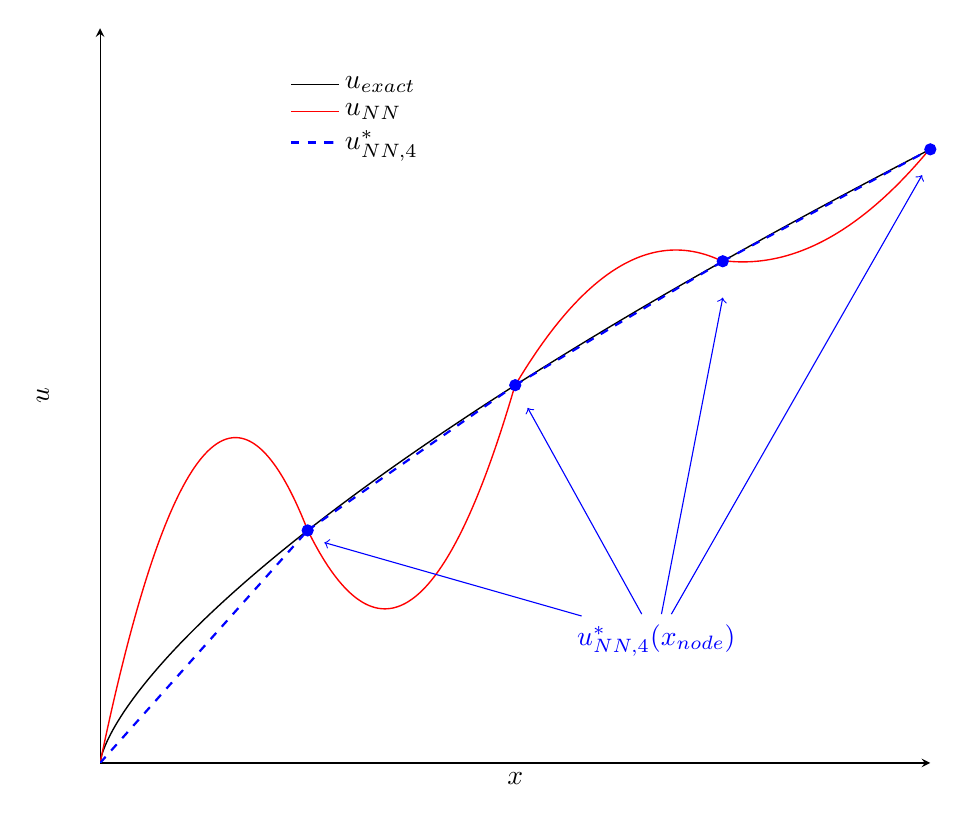
\begin{tikzpicture}
    \begin{axis}[
    xlabel = {$x$},
    xmin=0,
    xmax=10,
    ymin=0,
    ymax=6,
    ylabel = {$u$},
      height=0.9*\textwidth,
      width=1*\textwidth,
    axis lines=left,
    ticks=none,
%    grid=both,
	%xtick={0,0.25,...,1},
	%ytick={0,100},
    %yticklabels={0,$a$},
    y label style={at={(-0.05,0.5)}},
%    xticklabels={-3,-1,...,5},
%    ticks=xticklabels,
    legend columns = 1,
    legend style= {at={(0.4,0.95)},draw=none,fill=none,nodes={scale=1, transform shape}}, legend cell align={left}]
    ]    
    \tikzset{ dot/.style = {circle, fill, minimum size=3pt, inner sep=0pt, outer sep=0pt}, }
% exact 
\addplot[samples=500,color=black, smooth, line width=0.5, domain=0:10] {x^0.7};	
\addlegendentry{$u_{exact}$};

%% u_NN
\addplot[samples=500,color=red, smooth, line width=0.5, domain=0:2.5] {-x^2+3.26*x };
\addlegendentry{$u_{NN}$}
\addplot[samples=10,color=blue, smooth, dashed, domain=0:2.5, line width=0.8] {1.899/2.5*x};
\addlegendentry{$u^{*}_{NN,4}$ }
%
%
%%%%%%%% WE NEED TO PUT THE FIRST THREE PLOTS DIFFERENT TO OBTAIN THE CORRECT LEGEND IN THE PLOT
%
%%% u_NN
\addplot[samples=500,color=red, smooth, line width=0.5, domain=2.5:5] {0.743*(x^2)-5.097*x +10};
\addplot[samples=500,color=red, smooth, line width=0.5, domain=5:7.5] {-0.295*(x^2)+4.0918*x -10};
\addplot[samples=500,color=red, smooth, line width=0.5, domain=7.5:10] {0.182*(x^2)-2.818*x +15};

%% u_p
\draw[color=blue, smooth, dashed, line width=0.8] (2.5,1.899) -- (5,3.085);
\draw[color=blue, smooth, dashed, line width=0.8] (5,3.085) -- (7.5,4.097);
\draw[color=blue, smooth, dashed, line width=0.8] (7.5,4.097) -- (10,5.011);

%%points
\addplot[only marks,mark=*,blue,mark size=2pt] coordinates {(2.5,1.899)(5,3.085)(7.5,4.097)(10,5.011)};

    \tikzstyle{state}=[
        draw = white,
        thick,
        fill = white,
        minimum width=15mm, 
        minimum height=4mm
    ]

\node(G)[ state,  ] at (axis cs: 6.7,1.) {\textcolor{blue}{$u^{*}_{NN,4}(x_{node})$}};
%\node(G_aux1)[anchor = north, text width=1.0] at (axis cs: 1.65,31) {};
%\node(G_aux2)[anchor = north, text width=1.0] at (axis cs: 2,31) {};
    

%\node (G1) at (axis cs: 0.28175, 19){};
%\node (G2) at (axis cs: 1.25, 46.27){};
%\node (G3) at (axis cs: 2.21825, 36.05){};
%
%\draw[] (G1) node[above, blue] {};
%\draw[] (G2) node[above, blue] {};
%\draw[] (G3) node[above, blue] {};


\path[->, blue] (axis cs: 5.8,1.2) edge (axis cs:2.7,1.8);
\path[->, blue] (G) edge (axis cs:5.15,2.9);
\path[->, blue] (G) edge (axis cs:7.5,3.8);
\path[->, blue] (G) edge (axis cs:9.9,4.8);

\end{axis}
\end{tikzpicture}
\end{column}
%
\begin{column}{0.55\textwidth}
\begin{itemize}
\item[\tickNo]  Mesh based method
\item[\tickYes] Appropriate for low dimensions
\item[\tickYes] Allows exact integration $\&$ differentiation
\item[\tickNo]  It does not allow the use of autodiff
\item[\tickYes] Exists theory about its convergence
\end{itemize}
\end{column}
\end{columns}
\end{frame}
%%%%%%%%%%%%%%%%%%%%%%%%%%%%%%%%%%%%%%%%%%%%%%%%%%%%%%%%%%%%%%%%%%%%


\begin{frame}[t]{Numerical Results}
\only<1-1>{
\textbf{Piecewise-linear approximation:}

Mesh with four and ten elements. One Gauss point per element. $u_{exact}=x^{0.7}$.
%\vspace{0.5cm}

\begin{minipage}{.45\textwidth}
\begin{figure}[!htp]
\centering
\begin{tikzpicture}
%https://tex.stackexchange.com/questions/451704/tikz-position-of-an-imported-image
  \node[anchor=south west,inner sep=0] (image) at (0,0) {\begin{tikzpicture}
\begin{axis}[scale only axis, xlabel = $x$, ylabel = $u$, ytick pos=left, y label style={at={(-0.1,0.5)}}, legend style= {at={(0.3,0.95)}, fill=none,draw=none,nodes={scale=1.0, transform shape}}, legend cell align={left}, height=4cm, width=4cm, xmin=-0.2, ymin=0, xmax=10.2, ymax=5.5,samples=1000, xticklabel style={yshift=-3pt}, yticklabel style={xshift=-3pt}]
%\addlegendimage{only marks, mark size=4pt, mark=-, color=black} 
%\addlegendimage{only marks, mark size=4pt, mark=-, color=red}
\addplot [black, line width=1pt,domain=0:10] {x^0.7};
%\addlegendentry{\textcolor{black}{$u_{exact}$}}
\addplot[line width=0.7pt,color=red] %
	table[x=x ,y=u_pred]{Diapos/PDEs_with_NN/Figures/Alternatives//Data//data_Ritz_FD_4elem.csv};
%\addlegendentry{\textcolor{red}{$u_{NN}$ 4 elem}}
\addplot[line width=0.7pt,color=blue] %
	table[x=x ,y=u_pred]{Diapos/PDEs_with_NN/Figures/Alternatives//Data//data_Ritz_FD_10elem.csv};
%\addlegendentry{\textcolor{blue}{$u_{NN}$ 10 elem}}
% Legend
%\node[anchor = south] (Ua)at (3,4.5){\textcolor{red}{$u_{\varphi}$}};
%\node[anchor = south] at (3,4){\textcolor{black}{$u_{exact}$}};
\end{axis}
\end{tikzpicture}
};
  \begin{scope}[x={(image.south east)},y={(image.north west)}]
  \draw[<-, color=red] (0.3,0.35) -- (0.5,0.3) node[right, text width=0.925cm] {\textcolor{red}{$u^{*}_{NN,4}$}};
    \draw[<-, color=blue] (0.58,0.7) -- (0.5,0.8) node[above left, text width=1.09cm] {\textcolor{blue}{$u^{*}_{NN,10}$}};
  \draw[<-] (0.37,0.53) -- (0.3,0.6) node[above] {$u_{exact}$};
  \end{scope}
\end{tikzpicture}

 \end{figure}
\end{minipage}%
\hspace{1.5cm}
\begin{minipage}{.35\textwidth}
\vspace{0.9cm}
\begin{figure}[!htp]
\centering
\begin{tikzpicture}
%https://tex.stackexchange.com/questions/451704/tikz-position-of-an-imported-image
  \node[anchor=south west,inner sep=0] (image) at (0,0) {\input{Diapos/PDEs_with_NN/Figures/Alternatives/Graphics/Ritz_model_problem_1_FD_loss.tex}};
  \begin{scope}[x={(image.south east)},y={(image.north west)}]
%  \draw[<-, color=red] (0.355,0.26) -- (0.355,0.29) node[above] {\textcolor{red}{{\small $\mathcal{F}_{R}(u_{exact})$}}};
  \node[] at (0.37,0.3) (c) {\textcolor{black}{{\small $\mathcal{L}_{\mathcal{R}}(u_{exact})$}}};
  \draw[<-,red] (0.53,0.36) -- (0.6,0.75) node[above, text width=1.3cm] {\textcolor{red}{{\small $\mathcal{L}_{\mathcal{R}}(u^{*}_{NN,4})$}}};
  \draw[<-, color=blue] (0.61,0.36) -- (0.8,0.45) node[above, text width=1.5cm] {\textcolor{blue}{{\small $\mathcal{L}_{\mathcal{R}}(u^{*}_{NN,10})$}}};
  \end{scope}
\end{tikzpicture}

 \end{figure}
\end{minipage}%
}

 \only<2-2>{
\textbf{Adaptive integration:}

Mesh with four elements. Three Gauss points per element. $u_{exact}=x^{0.7}$.
%\vspace{0.5cm}

\begin{minipage}{.45\textwidth}
\begin{figure}[!htp]
\centering
\begin{tikzpicture}
%https://tex.stackexchange.com/questions/451704/tikz-position-of-an-imported-image
  \node[anchor=south west,inner sep=0] (image) at (0,0) {\begin{tikzpicture}
\begin{axis}[scale only axis, xlabel = $x$, ylabel = $u$, ytick pos=left, y label style={at={(-0.1,0.5)}}, legend style= {at={(0.3,0.95)}, fill=none,draw=none,nodes={scale=1.0, transform shape}}, legend cell align={left}, height=4cm, width=4cm, xmin=-0.2, ymin=0, xmax=10.2, ymax=5.5,samples=1000, xticklabel style={yshift=-3pt}, yticklabel style={xshift=-3pt}]
\addlegendimage{only marks, mark size=4pt, mark=-, color=black} 
\addlegendimage{only marks, mark size=4pt, mark=-, color=red}
\addplot [black, line width=2pt,domain=0:10] {x^0.7};
%\addlegendentry{\textcolor{black}{$u_{exact}$}}
\addplot[line width=0.7pt,color=red] %
	table[x=x ,y=u_pred]{Diapos/PDEs_with_NN/Figures/Alternatives//Data//data_Ritz_adaptive.csv};
%\addlegendentry{\textcolor{red}{$u_{NN}$}}
\end{axis}
\end{tikzpicture}
};
  \begin{scope}[x={(image.south east)},y={(image.north west)}]
  \draw[<-, color=red] (0.4,0.35) -- (0.55,0.3) node[below right] {\textcolor{red}{$u_{NN}$}};
  \draw[<-] (0.62,0.7) -- (0.45,0.8) node[above left] {$u_{exact}$};
  \end{scope}
\end{tikzpicture}

 \end{figure}
\end{minipage}%
\hspace{1.5cm}
\begin{minipage}{.35\textwidth}
\vspace{0.9cm}
\begin{figure}[!htp]
\centering
\begin{tikzpicture}
%https://tex.stackexchange.com/questions/451704/tikz-position-of-an-imported-image
  \node[anchor=south west,inner sep=0] (image) at (0,0) {\begin{tikzpicture}
\begin{axis}[scale only axis, xlabel = $Epoch$, ylabel = $Loss$, ytick pos=left, y label style={at={(-0.1,0.5)}}, x label style={at={(0.5,-0.15)}}, legend style= {at={(0.95,0.95)},draw=none,fill=none,nodes={scale=0.8, transform shape}}, legend cell align={left}, height=4cm, width=4cm, xmin=0.95, ymin=-2, xmax=40000, ymax=10, ytick = {8,-1.54}, xmode=log, xticklabel style={yshift=-3pt}, yticklabel style={xshift=-3pt}]
\addplot [black, dashed, line width=0.7pt,domain=0.99999:39900] {-1.54};
%\addlegendentry{Loss of exact solution}
\addplot[line width=0.8pt,color=red] %
	table[x=epoch ,y=loss]{Diapos/PDEs_with_NN/Figures/Alternatives//Data//loss_Ritz_adaptivity_treshold.csv};
%\addlegendentry{Loss of NN approximation.};

% Legend
%\node[anchor = south] (Ua)at (6,32){\textcolor{red}{$u_{approx}$}};
%\node[anchor = south] at (6,6){\textcolor{black}{$u_{exact}$}};

\end{axis}
\end{tikzpicture}
};
  \begin{scope}[x={(image.south east)},y={(image.north west)}]
  \draw[<-, color=black] (0.33,0.23) -- (0.6,0.45) node[above right] {\textcolor{black}{$\mathcal{L}_{\mathcal{R}}(u_{exact})$}};
  \draw[<-, color=red] (0.32,0.67) -- (0.6,0.85) node[above right] {\textcolor{red}{$\mathcal{L}_{\mathcal{R}}(u_{NN})$}};
  \end{scope}
\end{tikzpicture}

 \end{figure}
\end{minipage}%
 }
 
 \only<3-3>{
 \textbf{Regularization:}
 Minimization of the energy $\int_0^{10} \frac{1}{2}u'(x)^2+2u(x)\,dx+u(10)$ with $u(0)=0$ and mid-point rule. $u_{exact}=x^{2}$.
 \vspace{0.5cm}
% \begin{figure}[!htp]
% \centering
%    \begin{tikzpicture}
%https://tex.stackexchange.com/questions/451704/tikz-position-of-an-imported-image
\node at (0,0) {};
  \node[anchor=south west,inner sep=0] (image) at (0.05,0.03) {\begin{tikzpicture}
\begin{axis}[scale only axis, xlabel = $x$, ylabel = $u$, ytick pos=left, y label style={at={(-0.15,0.5)}}, legend style= {at={(0.3,0.95)}, fill=none,draw=none,nodes={scale=1.0, transform shape}}, legend cell align={left}, height=4cm, width=4cm, xmin=-0.2, ymin=-40, xmax=10.2, ymax=110,samples=10000, xticklabel style={yshift=-3pt}, yticklabel style={xshift=-3pt}]
\addlegendimage{only marks, mark size=4pt, mark=-, color=black} 
\addlegendimage{only marks, mark size=4pt, mark=-, color=red}
\addplot [black, line width=1pt,domain=0:10] {x^2};
%\addlegendentry{\textcolor{black}{$u_{exact}$}}
\addplot[line width=0.7pt,color=red] %
	table[x=x ,y=u_pred]{Diapos/PDEs_with_NN/Figures/Alternatives//Data//data_NoRegN50M10_sol.txt};
%\addlegendentry{\textcolor{red}{$u_{NN}$}}
\end{axis}
\end{tikzpicture}
};
  \begin{scope}[x={(image.south east)},y={(image.north west)}]
  \draw[<-, color=red] (0.27,0.3) -- (0.35,0.25) node[right] {\textcolor{red}{$u_{NN}$}};
  \draw[<-] (0.55,0.45) -- (0.65,0.4) node[below right] {$u_{exact}$};
  \end{scope}
\end{tikzpicture}

%    	\hspace{1cm}
%	\begin{tikzpicture}
%https://tex.stackexchange.com/questions/451704/tikz-position-of-an-imported-image
  \node[anchor=south west,inner sep=0] (image) at (0,0) {\begin{tikzpicture}
\begin{axis}[scale only axis, xlabel = $Epoch$, ylabel = $Loss$, ytick pos=left, y label style={at={(-0.1,0.5)}}, x label style={at={(0.5,-0.15)}}, legend style= {at={(0.95,0.95)},draw=none,fill=none,nodes={scale=0.8, transform shape}}, legend cell align={left}, height=4cm, width=4cm, xmin=0.95, xmax=30000, xmode=log, xticklabel style={yshift=-3pt}, yticklabel style={xshift=-3pt}]
%\addplot [red, dashed, line width=0.7pt,domain=0.99999:200000] {-666.67};
%\addlegendentry{Loss of exact solution}
\addplot[line width=0.8pt,color=black] %
	table[x=iter ,y=loss]{Diapos/PDEs_with_NN/Figures/Alternatives//Data//data_NoRegN50M10_R.txt};
%\addlegendentry{Loss $\mathcal{R}$};
\end{axis}
\end{tikzpicture}
};
  \begin{scope}[x={(image.south east)},y={(image.north west)}]
  \draw[<-] (0.95,0.7) -- (0.75,0.75) node[above left] {Loss $R$};
  \end{scope}
\end{tikzpicture}

%  \end{figure}
  
  \begin{minipage}{.45\textwidth}
\begin{figure}[!htp]
\centering
\begin{tikzpicture}
%https://tex.stackexchange.com/questions/451704/tikz-position-of-an-imported-image
\node at (0,0) {};
  \node[anchor=south west,inner sep=0] (image) at (0.05,0.03) {\begin{tikzpicture}
\begin{axis}[scale only axis, xlabel = $x$, ylabel = $u$, ytick pos=left, y label style={at={(-0.15,0.5)}}, legend style= {at={(0.3,0.95)}, fill=none,draw=none,nodes={scale=1.0, transform shape}}, legend cell align={left}, height=4cm, width=4cm, xmin=-0.2, ymin=-40, xmax=10.2, ymax=110,samples=10000, xticklabel style={yshift=-3pt}, yticklabel style={xshift=-3pt}]
\addlegendimage{only marks, mark size=4pt, mark=-, color=black} 
\addlegendimage{only marks, mark size=4pt, mark=-, color=red}
\addplot [black, line width=1pt,domain=0:10] {x^2};
%\addlegendentry{\textcolor{black}{$u_{exact}$}}
\addplot[line width=0.7pt,color=red] %
	table[x=x ,y=u_pred]{Diapos/PDEs_with_NN/Figures/Alternatives//Data//data_NoRegN50M10_sol.txt};
%\addlegendentry{\textcolor{red}{$u_{NN}$}}
\end{axis}
\end{tikzpicture}
};
  \begin{scope}[x={(image.south east)},y={(image.north west)}]
  \draw[<-, color=red] (0.27,0.3) -- (0.35,0.25) node[right] {\textcolor{red}{$u_{NN}$}};
  \draw[<-] (0.55,0.45) -- (0.65,0.4) node[below right] {$u_{exact}$};
  \end{scope}
\end{tikzpicture}

 \end{figure}
\end{minipage}%
\hspace{1.5cm}
\begin{minipage}{.35\textwidth}
\vspace{-0.25cm}
\begin{figure}[!htp]
\centering
\begin{tikzpicture}
%https://tex.stackexchange.com/questions/451704/tikz-position-of-an-imported-image
  \node[anchor=south west,inner sep=0] (image) at (0,0) {\begin{tikzpicture}
\begin{axis}[scale only axis, xlabel = $Epoch$, ylabel = $Loss$, ytick pos=left, y label style={at={(-0.1,0.5)}}, x label style={at={(0.5,-0.15)}}, legend style= {at={(0.95,0.95)},draw=none,fill=none,nodes={scale=0.8, transform shape}}, legend cell align={left}, height=4cm, width=4cm, xmin=0.95, xmax=30000, xmode=log, xticklabel style={yshift=-3pt}, yticklabel style={xshift=-3pt}]
%\addplot [red, dashed, line width=0.7pt,domain=0.99999:200000] {-666.67};
%\addlegendentry{Loss of exact solution}
\addplot[line width=0.8pt,color=black] %
	table[x=iter ,y=loss]{Diapos/PDEs_with_NN/Figures/Alternatives//Data//data_NoRegN50M10_R.txt};
%\addlegendentry{Loss $\mathcal{R}$};
\end{axis}
\end{tikzpicture}
};
  \begin{scope}[x={(image.south east)},y={(image.north west)}]
  \draw[<-] (0.95,0.7) -- (0.75,0.75) node[above left] {Loss $R$};
  \end{scope}
\end{tikzpicture}

 \end{figure}
\end{minipage}%
 }
 
\only<4-4>{
 \textbf{Regularization:}
 Minimization of the energy $\int_0^{10} \frac{1}{2}u'(x)^2+2u(x)\,dx+u(10)$ with $u(0)=0$ and mid-point rule. $u_{exact}=x^{2}$.
 \vspace{0.35cm}
 
\begin{minipage}{.45\textwidth}
\begin{figure}[!htp]
\centering
\begin{tikzpicture}
%https://tex.stackexchange.com/questions/451704/tikz-position-of-an-imported-image
\node at (0,0) {};
  \node[anchor=south west,inner sep=0] (image) at (0.02,0.03) {\input{Diapos/PDEs_with_NN/Figures/Alternatives/Graphics/Ritz_model_problem_2_Imp1_REG.tex}};
  \begin{scope}[x={(image.south east)},y={(image.north west)}]
  \draw[<-, color=red] (0.6,0.3) -- (0.7,0.25) node[right] {\textcolor{red}{$u_{NN}$}};
  \draw[<-] (0.78,0.67) -- (0.65,0.85) node[above] {$u_{exact}$};
  \end{scope}
\end{tikzpicture}

 \end{figure}
\end{minipage}%
\hspace{1.5cm}
\begin{minipage}{.35\textwidth}
\vspace{0.3cm}
\begin{figure}[!htp]
\centering
\begin{tikzpicture}
%https://tex.stackexchange.com/questions/451704/tikz-position-of-an-imported-image
  \node[anchor=south west,inner sep=0] (image) at (0,0) {\begin{tikzpicture}
\begin{axis}[scale only axis, xlabel = $Epoch$, ylabel = $Loss$, ytick pos=left, y label style={at={(-0.15,0.5)}}, legend style= {at={(0.7,0.95)},draw=none,fill=none,nodes={scale=0.8, transform shape}}, legend cell align={left}, height=4cm, width=4cm, xmin=0.95, xmax=15000, xmode=log, xticklabel style={yshift=-3pt}, yticklabel style={xshift=-3pt}]
%\addplot [red, dashed, line width=0.7pt,domain=0.99999:200000] {-666.67};
%\addlegendentry{Loss of exact solution}
\addplot[line width=0.8pt,color=black] %
	table[x=iter ,y=loss]{Diapos/PDEs_with_NN/Figures/Alternatives//Data//data_RegN50M10_R.txt};
%\addlegendentry{Loss $\mathcal{R}$};

% Legend
%\node[anchor = south] (Ua)at (6,32){\textcolor{red}{$u_{approx}$}};
%\node[anchor = south] at (6,6){\textcolor{black}{$u_{exact}$}};

\end{axis}
\end{tikzpicture}
};
  \begin{scope}[x={(image.south east)},y={(image.north west)}]
  \draw[<-] (0.7,0.57) -- (0.55,0.85) node[above left] {Loss $R$};
  \end{scope}
\end{tikzpicture}

 \end{figure}
\end{minipage}%
 }
 \end{frame}


\begin{frame}{Deep Neural Networks for Solving PDEs}
\begin{itemize}
\item Quadrature errors appear when solving PDEs using DL methods.
\vspace{0.5cm}
\item Selecting an adequate quadrature rule is critical.
\vspace{0.5cm}
\item For high dimensions Monte Carlo is adequate.
\vspace{0.5cm}
\item We propose adaptive integration for low dimensions.
\end{itemize}
\end{frame}